% Generated PDF baseline(s):
%   ../fig6.2.pdf
% Note: this source already differed from that checked-in PDF before centralization.
% ============================================================================
% EDITABLE FIGURE PARAMETERS
% The document-class options below set the base font and cropped-page margin.
% Example: change 12pt to 11pt for all inherited text, or border=2pt to
% border=4pt for a larger white margin. Keep the current values to reproduce
% the dissertation figure exactly.
%
% Colors declared with \definecolor and pre-existing \tikzset blocks are also
% centralized appearance constants. Edit their values in this preamble only.
% ============================================================================
\documentclass[tikz,border=3pt]{standalone}

\pdfinfoomitdate=1
\pdftrailerid{}
\pdfsuppressptexinfo=15

\usepackage{amsmath}
\usetikzlibrary{arrows.meta,positioning,shapes.geometric}


% --- Centralized render constants used by the figure body ---
% Text-node constants: font, padding, border, fill, anchor, and relative placement.
% Example: inside a node macro, change inner sep=3pt to 4pt or font=\normalsize to font=\small.
\long\def\FluidraFigureNodeA{\node[title,text=red!55!black]}
\long\def\FluidraFigureNodeB{\node[failed]}
\long\def\FluidraFigureNodeC{\node[failed,right=7mm of sparse]}
\long\def\FluidraFigureNodeD{\node[failed,right=7mm of bn]}
\long\def\FluidraFigureNodeE{\node[failed,right=7mm of mse]}
\long\def\FluidraFigureNodeF{\node[failed,right=7mm of argmax]}
\long\def\FluidraFigureNodeG{\node[title,text=blue!55!black]}
\long\def\FluidraFigureNodeH{\node[safe]}
\long\def\FluidraFigureNodeI{\node[safe,right=7mm of raw]}
\long\def\FluidraFigureNodeJ{\node[safe,right=7mm of expanded]}
\long\def\FluidraFigureNodeK{\node[safe,right=7mm of gn]}
\long\def\FluidraFigureNodeL{\node[safe,right=7mm of scores]}
\long\def\FluidraFigureNodeM{\node[support,below=7mm of expanded]}
\long\def\FluidraFigureNodeN{\node[support,below=7mm of gn]}
\long\def\FluidraFigureNodeO{\node[support,below=7mm of scores]}

% Path constants: arrow shape, color, dash pattern, and stroke width.
% Example: inside a path macro, change line width=0.8pt to 1pt or >=Latex to >=Stealth.
\long\def\FluidraFigurePathA{\draw[flow]}
\long\def\FluidraFigurePathB{\draw[flow]}
\long\def\FluidraFigurePathC{\draw[flow]}
\long\def\FluidraFigurePathD{\draw[flow]}
\long\def\FluidraFigurePathE{\draw[flow]}
\long\def\FluidraFigurePathF{\draw[flow]}
\long\def\FluidraFigurePathG{\draw[flow]}
\long\def\FluidraFigurePathH{\draw[flow]}
\long\def\FluidraFigurePathI{\draw[flow]}
\long\def\FluidraFigurePathJ{\draw[flow]}
\long\def\FluidraFigurePathK{\draw[flow]}

% Position constants: absolute or axis-relative locations for annotations and paths.
% \FluidraFigurePositionA controls one location. Example: adjust either coordinate below to move it.
\def\FluidraFigurePositionA{0,4.75}
% \FluidraFigurePositionB controls one location. Example: adjust either coordinate below to move it.
\def\FluidraFigurePositionB{0,3.45}
% \FluidraFigurePositionC controls one location. Example: adjust either coordinate below to move it.
\def\FluidraFigurePositionC{0,1.65}
% \FluidraFigurePositionD controls one location. Example: adjust either coordinate below to move it.
\def\FluidraFigurePositionD{0,0.35}
\begin{document}
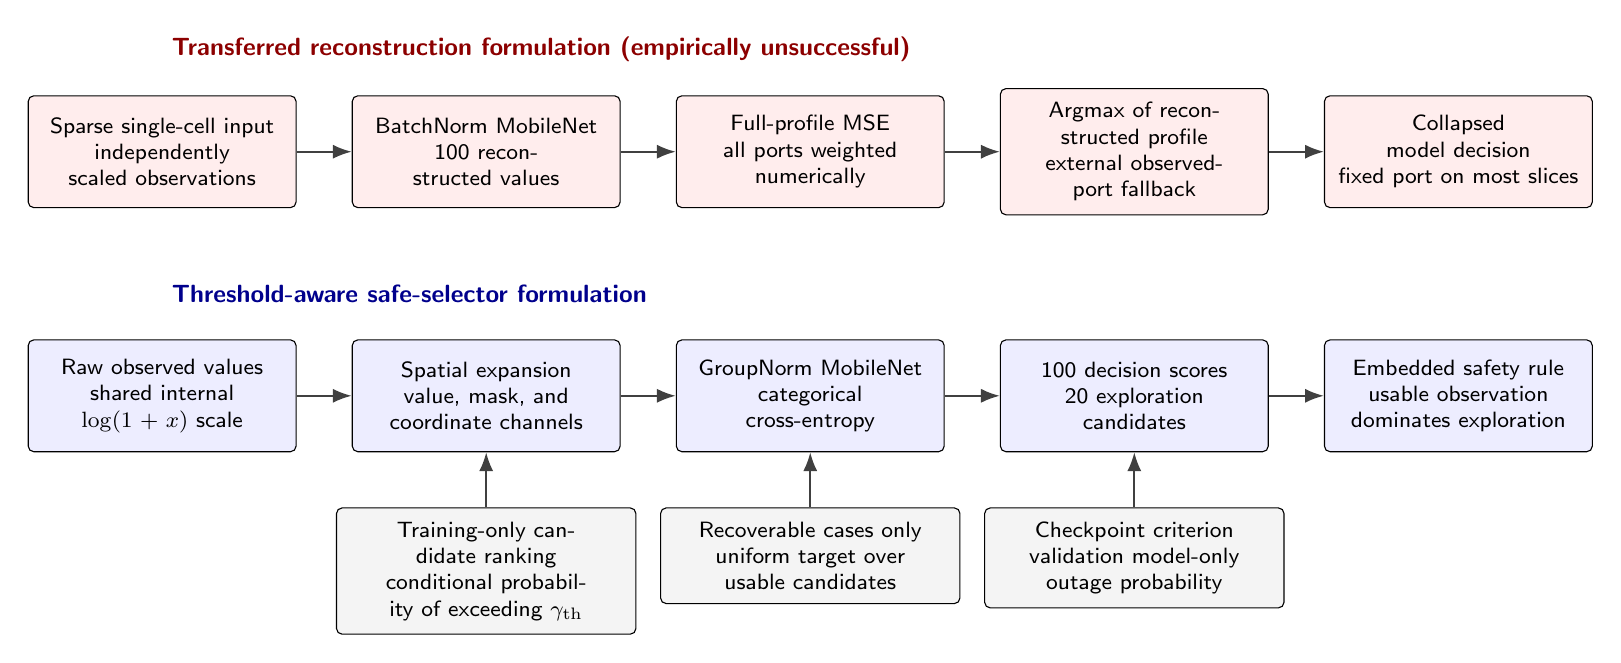
\begin{tikzpicture}[
    font=\sffamily\footnotesize,
    >=Latex,
    flow/.style={-{Latex[length=2.4mm]},line width=0.75pt,draw=black!75},
    box/.style={draw=black,rounded corners=2pt,align=center,
        minimum height=1.42cm,text width=3.05cm,inner sep=5pt},
    failed/.style={box,fill=red!7},
    safe/.style={box,fill=blue!7},
    support/.style={box,fill=gray!9,minimum height=1.18cm,text width=3.45cm},
    title/.style={font=\sffamily\bfseries\small,anchor=west}
]

\FluidraFigureNodeA at (\FluidraFigurePositionA) {Transferred reconstruction formulation (empirically unsuccessful)};
\FluidraFigureNodeB (sparse) at (\FluidraFigurePositionB) {Sparse single-cell input\\independently scaled observations};
\FluidraFigureNodeC (bn) {BatchNorm MobileNet\\100 reconstructed values};
\FluidraFigureNodeD (mse) {Full-profile MSE\\all ports weighted numerically};
\FluidraFigureNodeE (argmax) {Argmax of reconstructed profile\\external observed-port fallback};
\FluidraFigureNodeF (collapse) {Collapsed model decision\\fixed port on most slices};
\FluidraFigurePathA (sparse) -- (bn);
\FluidraFigurePathB (bn) -- (mse);
\FluidraFigurePathC (mse) -- (argmax);
\FluidraFigurePathD (argmax) -- (collapse);

\FluidraFigureNodeG at (\FluidraFigurePositionC) {Threshold-aware safe-selector formulation};
\FluidraFigureNodeH (raw) at (\FluidraFigurePositionD) {Raw observed values\\shared internal $\log(1+x)$ scale};
\FluidraFigureNodeI (expanded) {Spatial expansion\\value, mask, and coordinate channels};
\FluidraFigureNodeJ (gn) {GroupNorm MobileNet\\categorical cross-entropy};
\FluidraFigureNodeK (scores) {100 decision scores\\20 exploration candidates};
\FluidraFigureNodeL (decision) {Embedded safety rule\\usable observation dominates exploration};
\FluidraFigurePathE (raw) -- (expanded);
\FluidraFigurePathF (expanded) -- (gn);
\FluidraFigurePathG (gn) -- (scores);
\FluidraFigurePathH (scores) -- (decision);

\FluidraFigureNodeM (ranking) {Training-only candidate ranking\\conditional probability of exceeding $\gamma_{\mathrm{th}}$};
\FluidraFigureNodeN (recoverable) {Recoverable cases only\\uniform target over usable candidates};
\FluidraFigureNodeO (checkpoint) {Checkpoint criterion\\validation model-only outage probability};
\FluidraFigurePathI (ranking.north) -- (expanded.south);
\FluidraFigurePathJ (recoverable.north) -- (gn.south);
\FluidraFigurePathK (checkpoint.north) -- (scores.south);

\end{tikzpicture}
\end{document}
